% !TEX root = DesignDocument.tex


\chapter{User Documentation}

\section{User Guide}

The following is the user guide for the DanceSoft project:

\subsection{Entering the Software}
Login page:\\
When the user first logs into the system the user is prompted with a log in window where they can enter their user name or pass word for the system. If the user enters the wrong password then the system pops up a dialog and tells the user to reenter there password. The default user name for a new user is the name used to enter the system. So if I enter a new teacher named Marcus Berger then the default user name is Marcus Berger. The default password is rcdance, both the user name and password can be changed using the change functions in the personal section of the teacher landing page.\\

\begin{figure}
  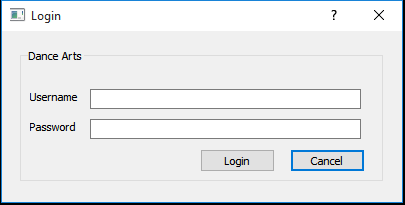
\includegraphics[width=\linewidth]{pics/userGuide/login.png}
  \caption{Log in page}
  \label{fig:User doc: log in}
\end{figure}

Landing Selection:\\
After the user logs in they can select which of the two landing pages, Admin or Teacher that they want to go to. If the user does not have admin permissions the user will be blocked from going to the Admin Landing page.\\

\subsection{Admin Landing}
Once an admin has logged in they can select the admin landing page to be taken to a variety of functions listed below. 
In the main page the user has four options for type of functions to choose from employee, student, class, and billing.\\

\begin{figure}
  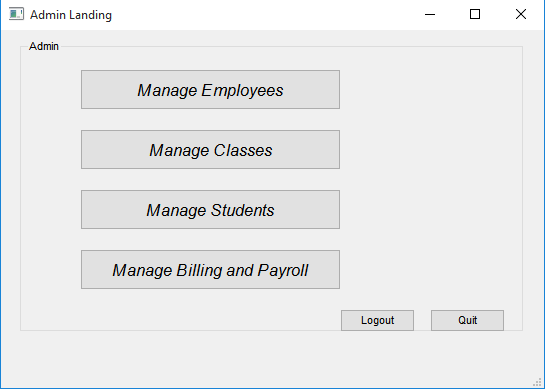
\includegraphics[width=\linewidth]{pics/userGuide/admin_landing.png}
  \caption{Admin Main Page}
  \label{fig:User doc: Admin Landing}
\end{figure}

\subsubsection{Manage Employees} 
When the user clicks on manage employee they are given a set of buttons that they can choose from.\\

Search Teacher:\\
When the user selects search teacher, the system will bring up a window that displays the teachers in the system. The user can then type a teacher's name into the search bar and the field will display the teachers that names contain the entered value. If the user is looking for an exact match then they can check the "exact check box. After the user conducts a search, they can click the refresh button to bring back the full list of teachers in the database.

By clicking the advanced search button the user can further refine the search value, the advanced search dialog is accessed by clicking the advanced search button. Advanced search allows the user to to search for teachers by id, name, phone numbers, or date of birth.

One the users desired teacher is found the user can click on the name in the main window and select a details button to view all the information for that teacher.  In the details window the user is able to change the information for an entry and submit the updates to the system.\\

\begin{figure}
  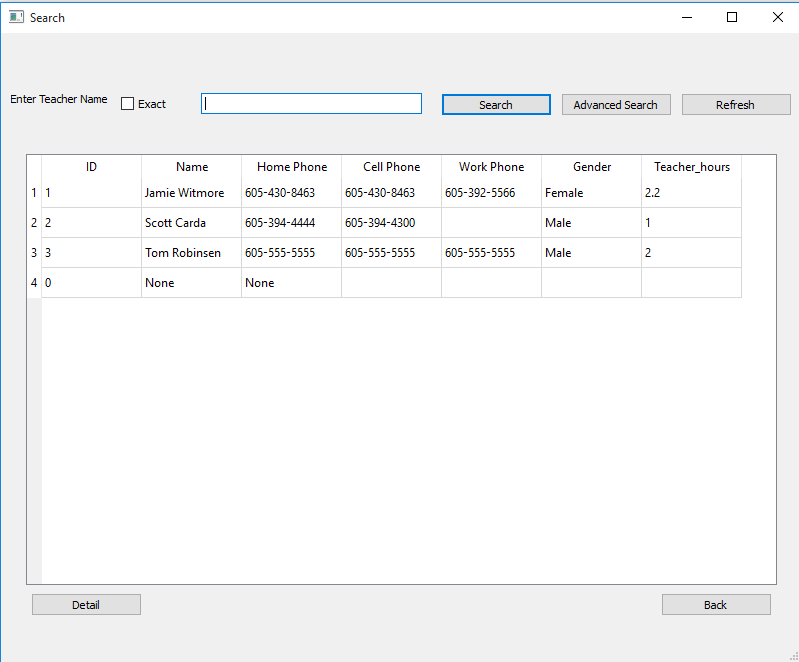
\includegraphics[width=\linewidth]{pics/userGuide/teacherSearch.png}
  \caption{Teacher Search Window}
  \label{fig:User doc: Teacher Search}
\end{figure}

Show Admin List:\\
On the main admin page the user can select the admin list button. This will display a text list of admins for the system. The window contains a search bar to refine the list if the user is looking for a specific entry. The page contains a details button which will allow the user to view the full details of the entry. The add button allows the user to select a teacher in the system and give them admin permissions.  The remove button allows the user to remove admin permissions from the system, this however does not remove the teacher from the system.\\

Update Teacher Information:\\
The update teacher button on the admin employee page, allows the user to select a teacher in the system and one selected a form will be populated. The user can then change any of the fields and submit the updates to the systems database.\\ 

\begin{figure}
  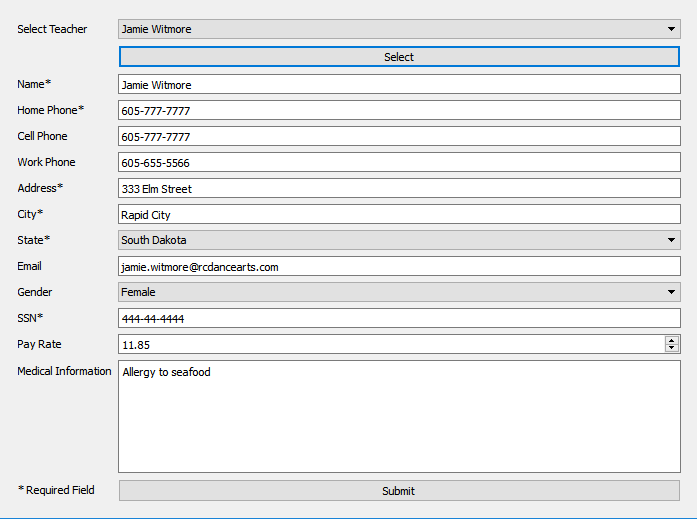
\includegraphics[width=\linewidth]{pics/userGuide/updateTeacher.png}
  \caption{Update Teacher Form}
  \label{fig:User doc: Teacher Update}
\end{figure}

Enter Teacher Hours:\\
Another button on the admin landing page is "Enter Teacher Hours". The user is able to select a teacher and a dialog pops up. The user is then able to view the selected teachers hours in each pay rate and change them if the user so chooses. The gross wage is then calculated and displayed to the user.\\

\begin{figure}
  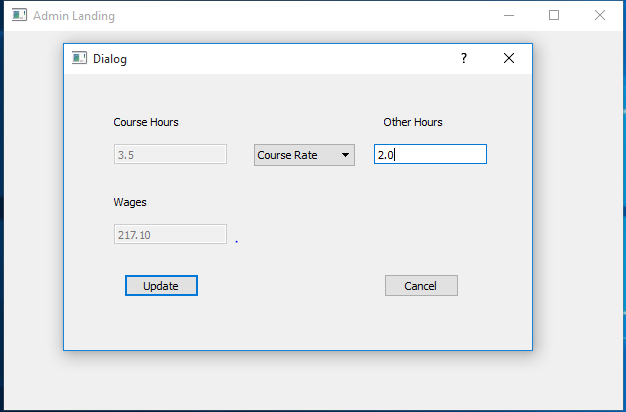
\includegraphics[width=\linewidth]{pics/userGuide/hours.png}
  \caption{The Admin Hours Page}
  \label{fig:User doc: Enter Hours}
\end{figure} 

Assign Teacher to Class:\\
This button bring up the assign teacher window. From here the user is able to select a class name, if the class is currently assigned to a teacher a dialog box will pop up asking the user if they would like to reassign the class to a different teacher. If the user selects yes or if the selected class is currently not assign to a teacher a list of teachers available at the class time will pop up and the user can select a teacher to assign to the class.\\

\begin{figure}
  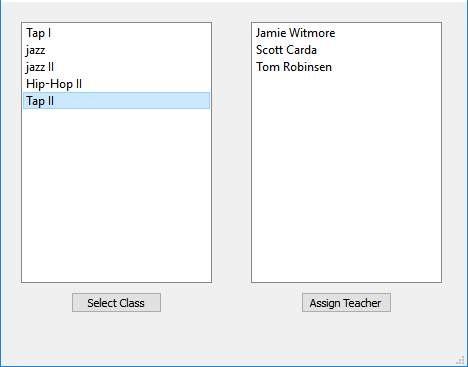
\includegraphics[width=\linewidth]{pics/userGuide/assignClass.png}
  \caption{Assign Class Window}
  \label{fig:User doc: Assign Class}
\end{figure} 

Teaching History:\\
The user is able to select a teacher and press the history button, this brings up a list of all the classes that teacher has taught, excluding the current semesters classes.\\

\begin{figure}
  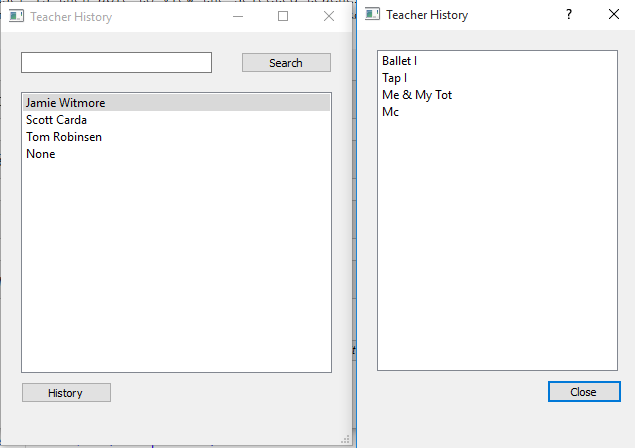
\includegraphics[width=\linewidth]{pics/userGuide/history.png}
  \caption{Teacher History}
  \label{fig:User doc: Teacher History}
\end{figure} 

Enter New Teacher:\\
This button ups a form where the user can enter the fields for a new teacher. Once all the required fields are filled out the user can submit the teacher to the system. The required fields are name, date of birth, home phone, address fields, gender, and SSN. When the submit button is clicked, the user will be able to review the entry before submitting it to the system.\\

Remove Teacher\\
The user is able to select the name of a teacher and remove the selected teacher from the system. This removal is complete, this means that if the user removes a teacher it will completely remove all the data from the system connected to that teacher. This includes classes, teacher data, and hours.\\

\subsubsection{Manage Classes}

View Classes\\
This button allows the user to search classes like in the teacher search explained above. The general functionality is the same, the user is able to search by class name and refresh the view window after a search. The user can check the exact button if they wish to look only for what they entered. The Advanced search button allows the user to search for classes based on id, name location and time. Once the desired class is found the user can select a class and press the details button in order to view the full details for a course. Within this details page the user can modify the information and send updates to the system.\\


\begin{figure}
  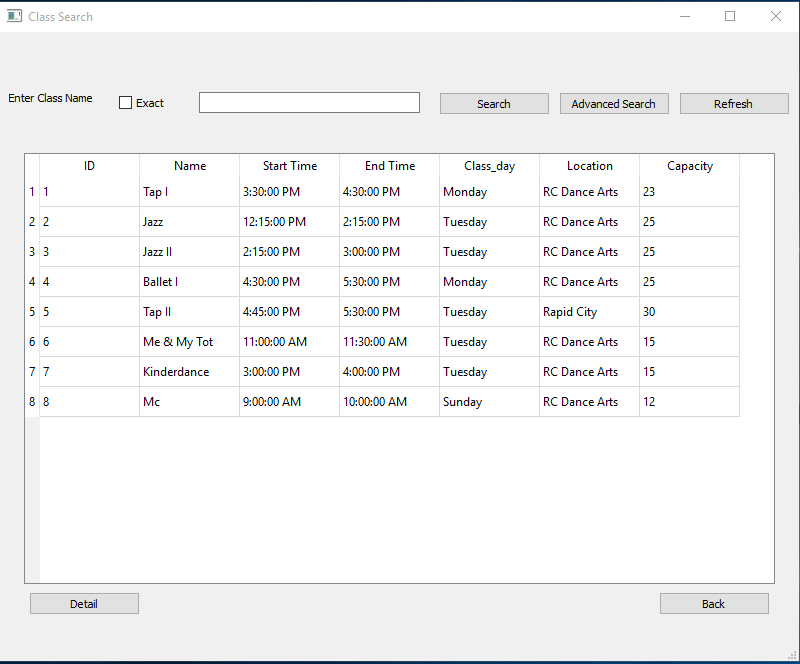
\includegraphics[width=\linewidth]{pics/userGuide/classSearch.png}
  \caption{Class Search Window}
  \label{fig:User doc: Class Search}
\end{figure}

Add a Class:\\
A form will pop up where the user can enter in all the information needed to add a class. Once the user has entered in all the information and clicked submit a dialog will pop up where the user can check and confirm the submission. Selecting "Add New Location" in the location drop down will pop up a dialog box which will allow the user to enter in a new location for the class, the user can also select a location that already exist in the system.\\

Remove Class:\\
The user is able to select the name of a class and remove the selected class from the system. This removal is complete, this means that if the user removes a class it will completely remove all the data from the system connected to that class. This includes class data, removal from schedules, removal from any billing calculations, and any pending registrations\\

Set Semester:\\
Allows the user to select the current semester in the system or add a new semester.

\begin{figure}
  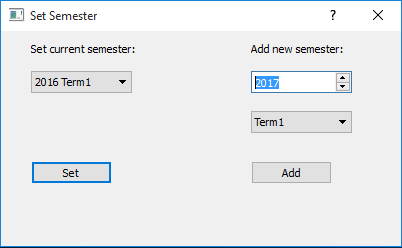
\includegraphics[width=\linewidth]{pics/userGuide/setSemester.png}
  \caption{Set Semester Window}
  \label{fig:User doc: Set Semester}
\end{figure}

\subsubsection{Manage Students}

Search Students:\\

When the user selects search student, the system will bring up a window that displays the students in the system. The user can then type a student's name into the search bar and the field will display the students that names contain the entered value. If the user is looking for an exact match then they can check the "exact check box. After the user conducts a search, they can click the refresh button to bring back the full list of students in the database.

By clicking the advanced search button the user can further refine the search value, the advanced search dialog is accessed by clicking the advanced search button. Advanced search allows the user to to search for students by id, name, phone, guardian or date of birth.

One the users desired student is found the user can click on the name in the main window and click a details button to view all the information for that student.  In the details window the user is able to change the information for an entry and submit the updates to the system.\\

\begin{figure}
  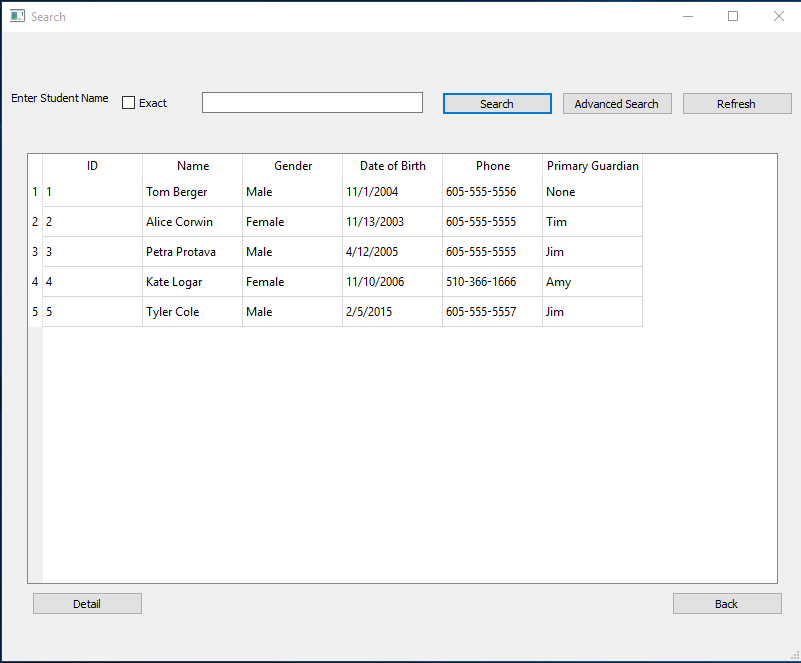
\includegraphics[width=\linewidth]{pics/userGuide/searchStudents.png}
  \caption{Student Search Window}
  \label{fig:User doc: Student Search}
\end{figure}


Student Credits:\\
This button will pull up a window where the user can select a students name and their credit amount within the system will be displayed. The user can then update the credit amount for that student. The credits are not factored into any student billing calculations. This is in accordance with the Academy of Dances Arts refund and credit policy as the credits and refund distribution is up to the users of the system. One the credits have been used the user must reset the reset the students credits to zero.\\

\begin{figure}
  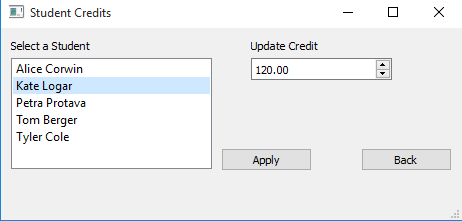
\includegraphics[width=\linewidth]{pics/userGuide/credits.png}
  \caption{Student Credit Window}
  \label{fig:User doc: Student Credits}
\end{figure}

Add/Remove Student:\\
This button brings up a window that allows the user to select a class. Once a class is selected the students currently registered will appear along with their class approval status. User can then select a student name and either click the add button to set the approval to one meaning the student is approved to take the class. A user can also remove the student which sets the approval to negative one meaning rejected. An approval of zero means the students registration is pending.

This function was created for the student interface links, however this set of functions were dropped so this function was left in at the request of the project's initial client Dr. Jeff McGough, so a future iteration of the project could see it. However in the projects current state this window serves no real overall purpose and should not be used by any users of the software. Anyone wishing to do student registration should do so through the student registration function explained below.\\


\begin{figure}
  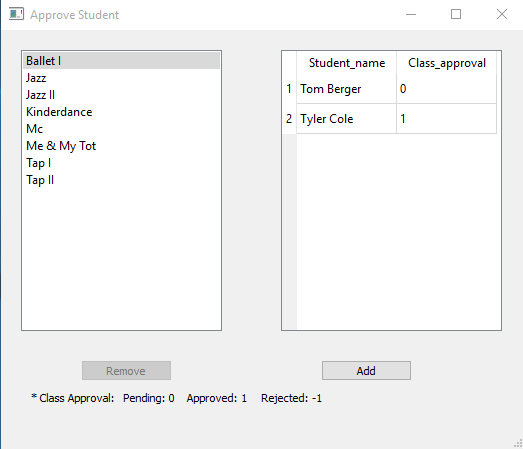
\includegraphics[width=\linewidth]{pics/userGuide/Addstu.png}
  \caption{First Student Registration}
  \label{fig:User doc: First Student Registration}
\end{figure}

Registration:\\
The user is able search for a preexisting and select a student. The user can then click the "Update" button to bring up the details of that student, the user can then change and update the student's information in the system.  Once the updates are made or if there are no information updates the user can click the "list" button and bring up a list of classes the student is currently registered for and the classes the student can register for. Classes can be dropped by selecting the class and clicking the drop button. Classes can be added from the pending class section using the add button.

Back on the student list window instead of clicking the "Update" button, the user can click the "Add" Button and enter in a new students information. If the  new students guardian is not in the system the user can click "Add Primary" to add the student's primary guardian. If the student needs a new secondary guardian the user can click the "Add Secondary" button and add another guardian to the system.  Once all the information for the student has been added the user can click the "Add" button to finalize the student.

\begin{figure}
  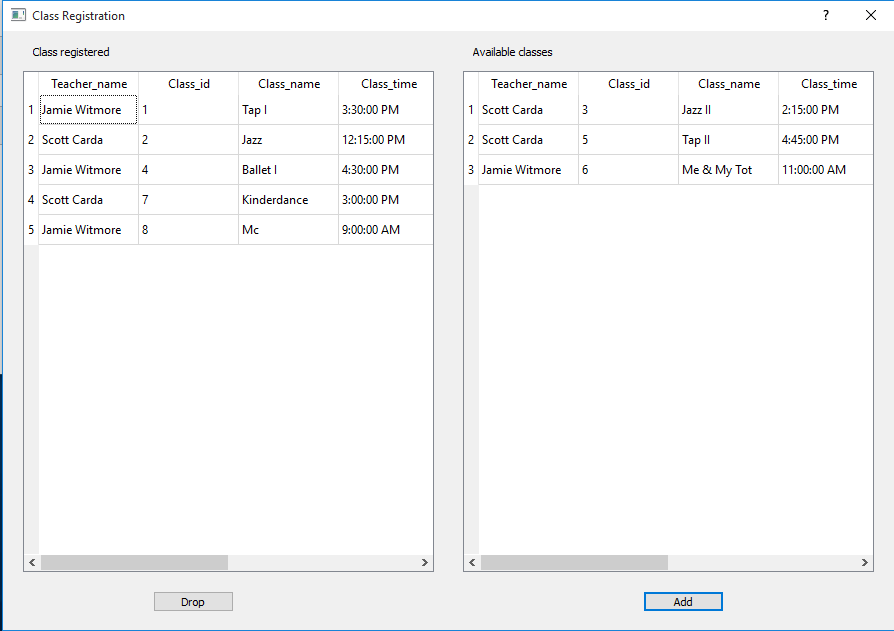
\includegraphics[width=\linewidth]{pics/userGuide/studentReg.png}
  \caption{Current Student Registration Window}
  \label{fig:User doc: Student Registration}
\end{figure}

\begin{figure}
  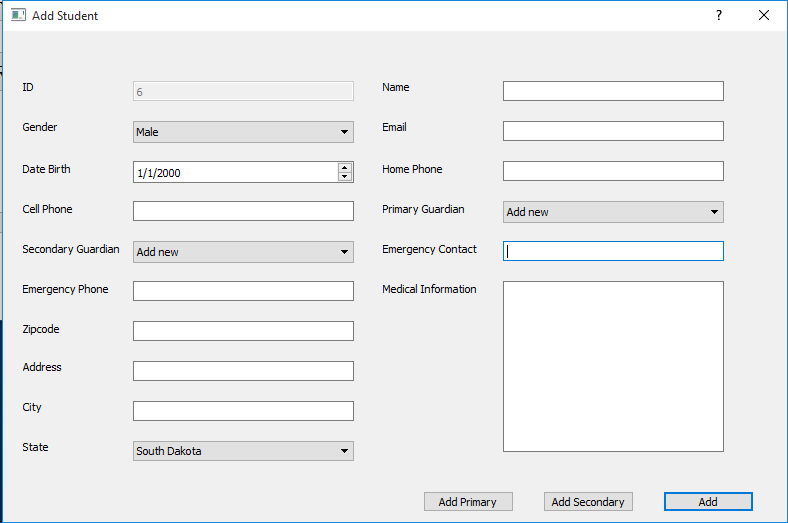
\includegraphics[width=\linewidth]{pics/userGuide/AddStudent.png}
  \caption{Add New Student Window}
  \label{fig:User doc: Add Student}
\end{figure}

Remove Student:\\
The user is able to select the name of a student using a search bar and remove the selected student from the system. This removal is complete, this means that if the user removes a student it will completely remove all the data from the system connected to that student. This includes class data, removal from schedules, removal from any billing calculations, any pending registrations, and if no other students such as sibling are connected to an address or a guardian the address and/or guardians will be removed as well. Any remove functions should be done with caution\\

\subsubsection{Manage Billing}
These functions are the general billing function for this version of the software ane allow the user to handle the base level billing functionality of the DanceSoft project.\\

Enter Partial Payment:\\
The User is able to search for a student and select them. When the user selects a student that is making a payment a window will appear where the user can type in the amount paid by the student. The type of payment is selected from a drop down menu, this value is used in the billing history to display how the student paid. The last combo box allows the user to select the term in which the payment was made. The payment is processed when the user clicks "Confirm."\\

\begin{figure}
  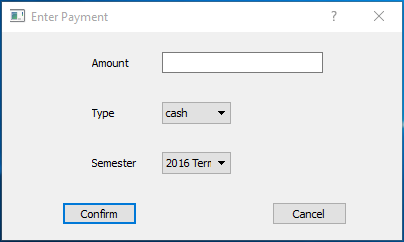
\includegraphics[width=\linewidth]{pics/userGuide/partPay.png}
  \caption{Partial Payment Window} 
  \label{fig:User doc: Partial Payment}
\end{figure}
  
Enter Full Payment:\\
Enter full payment works the same way as partial payment the user is able to search for an select a student, however instead of entering a payment by clicking the button the students owed amount will be set to zero.\\

Enter Teacher Pay Rate:\\
The Enter Teacher Pay Rate button opens up a window where the user can select a teacher. Once a teacher is selected the user can open the pay rate window. From the pay rate window the user can enter a new pay rate for the current teacher and the amount that pay rate is worth. The user can them add the pay rate to the system by clicking the "Add" button. If the user chooses to update the pay rate the user can select the rate they wish to update from the drop down menu and change the value in the box. The update is submitted by clicking the update button. Currently the added pay rates are for that teacher, but the course rate is the same among all teachers. Future versions should add the ability to have different course rates for each teacher.\\\

\begin{figure}
  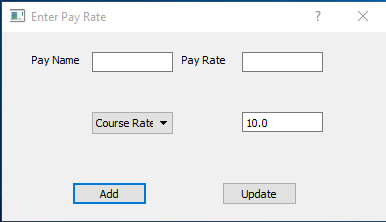
\includegraphics[width=\linewidth]{pics/userGuide/enterPay.png}
  \caption{Enter Pay Rate Window} 
  \label{fig:User doc: Enter Pay Rate}
\end{figure}

Student Balance:\\
The user selects a student and can clicks the "Statement" button. The students statement will produce a name, the current semester, the classes taken that semester, the total money paid, due, and the remaining balance. The user can print out the statement as well if needed.\\

\begin{figure}
  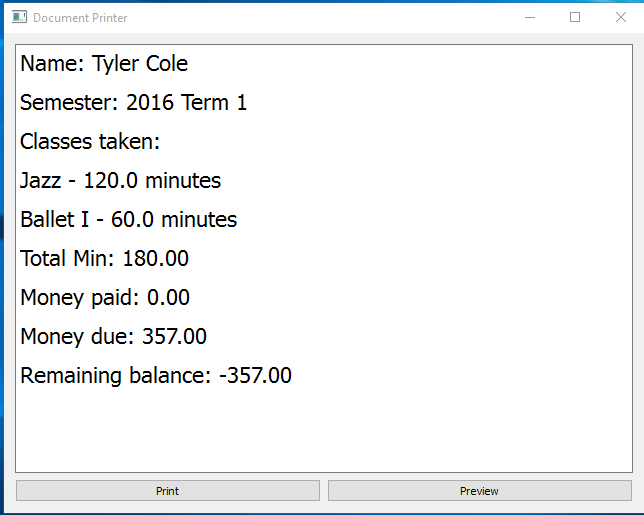
\includegraphics[width=\linewidth]{pics/userGuide/stuBalence.png}
  \caption{Student Balance Window} 
  \label{fig:User doc: Student Balance}
\end{figure}

Billing History:\\
When the user clicks the "Billing History" button, a window appears where the users can search for and select a student. Once a student is selected the user can click the statement button and produce the payment list for a student. The payment list contains the name of the student, the term the payment was made for, the amount paid, and the date the payment was made. The user can print the statement if they want to using the print button.  

\begin{figure}
  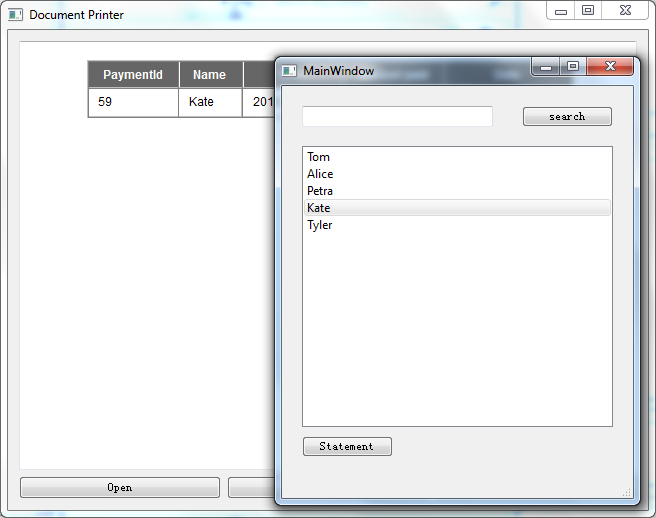
\includegraphics[width=\linewidth]{pics/userGuide/billHistory.png}
  \caption{Student Billing History} 
  \label{fig:User doc: Billing History}
\end{figure}

Tuition Rates and Fees:\\
The user is able to view all the tuition rates in the system and update them if need be, by changing the values of in the boxes. The user can also add and remove tuition rates as well. In the fee window the user can add a fee update a fee in the system and remove a fee it they so choose. However as of this version of the project none of the fees are factored in to any of the calculations. In future versions the project should be able to connect the fees to billing calculations. The tuition rates are based on the amount of minutes and they in turn determine the amount a student owes. If these are changed or remove it could mess with the way the system does billing for the Academy. Handle with caution. In future iterations teams should be able to better connect these systems.

\begin{figure}
  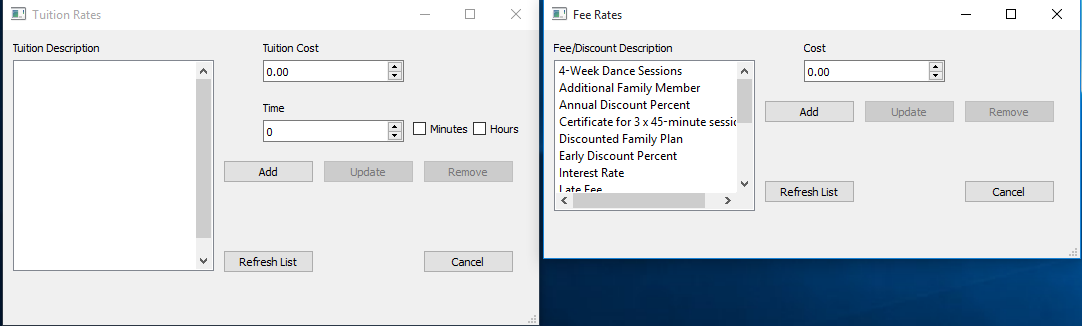
\includegraphics[width=\linewidth]{pics/userGuide/tuitAndFees.png}
  \caption{Tuition and Fees} 
  \label{fig:User doc: Tuition and Fees}
\end{figure}


\subsection{Teacher Landing}

\subsubsection{Student Options}

Search Students:\\
When the user selects search student, the system will bring up a window that displays the students in the system. The user can then type a student's name into the search bar and the field will display the students that names contain the entered value. If the user is looking for an exact match then they can check the "exact check box. After the user conducts a search, they can click the refresh button to bring back the full list of students in the database.

By clicking the advanced search button the user can further refine the search value, the advanced search dialog is accessed by clicking the advanced search button. Advanced search allows the user to to search for students by id, name, phone, guardian or date of birth.

One the users desired student is found the user can click on the name in the main window and click a details button to view all the information for that student.  In the details window the user is able to change the information for an entry and submit the updates to the system.\\

\begin{figure}
  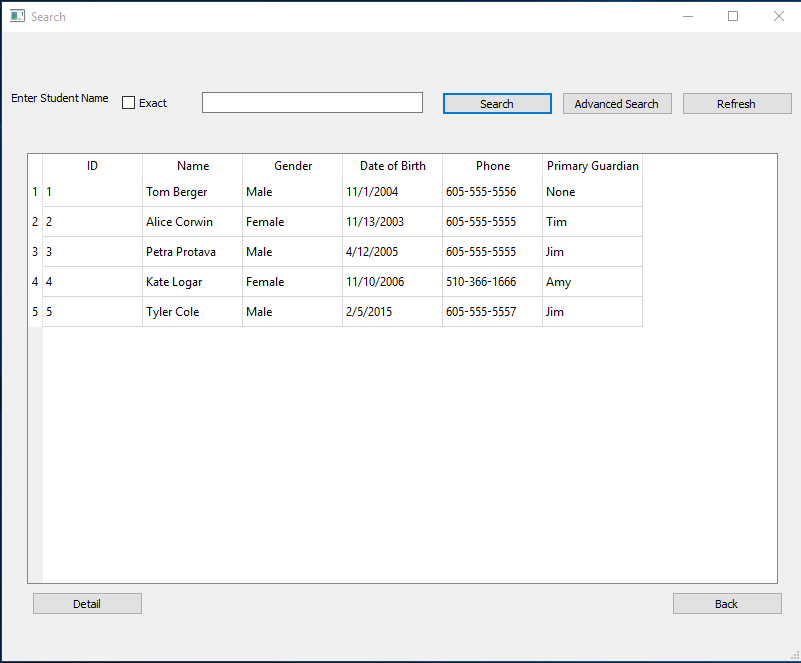
\includegraphics[width=\linewidth]{pics/userGuide/searchStudents.png}
  \caption{Student Search Window}
  \label{fig:User doc: Student Search}
\end{figure}

Add to Class:\\
This button brings up a window that allows the user to select a class. Once a class is selected the students currently registered will appear along with their class approval status. User can then select a student name and either click the add button to set the approval to one meaning the student is approved to take the class. A user can also remove the student which sets the approval to negative one meaning rejected. An approval of zero means the students registration is pending.

This function was created for the student interface links, however this set of functions were dropped so this function was left in at the request of the project's initial client Dr. Jeff McGough, so a future iteration of the project could see it. However in the projects current state this window serves no real overall purpose and should not be used by any users of the software. Anyone wishing to do student registration should do so through the student registration function explained below.\\

Student Schedule:\\
This button allows the user to pull up a window where they can select a student and view there class schedule. The user can also print out their schedule by pressing the print button. The schedule is design to only display the times that the student is in a class.\\

\begin{figure}
  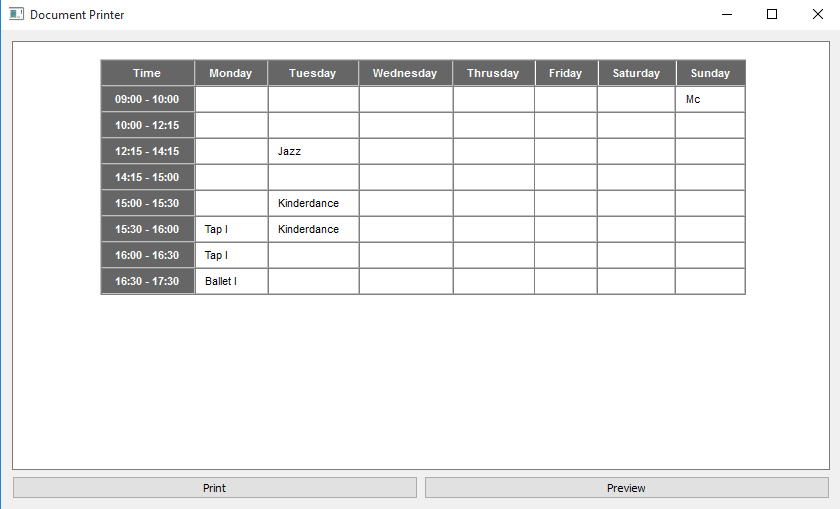
\includegraphics[width=\linewidth]{pics/userGuide/studentSchedule.png}
  \caption{Student Schedule Window}
  \label{fig:User doc: Student Schedule}
\end{figure}


\subsubsection{Class Options}
This section contains the class related function that a teacher may need to manage their day to day activities.

View Classes:\\
This button allows the user to search classes like in the teacher search explained in the admin section. The general functionality is the same, the user is able to search by class name and refresh the view window after a search. The user can check the exact button if they wish to look only for what they entered. The Advanced search button allows the user to search for classes based on id, name location and time. Once the desired class is found the user can select a class and press the details button in order to view the full details for a course. Within this details page the user can modify the information and send updates to the system.\\


Class Schedule:\\
This button allows the user to pull up a window where they can select a teacher and view there teaching schedule. The user can also print out their schedule by pressing the print button. The schedule is design to only display the times that the teacher is teaching a class.\\

\begin{figure}
  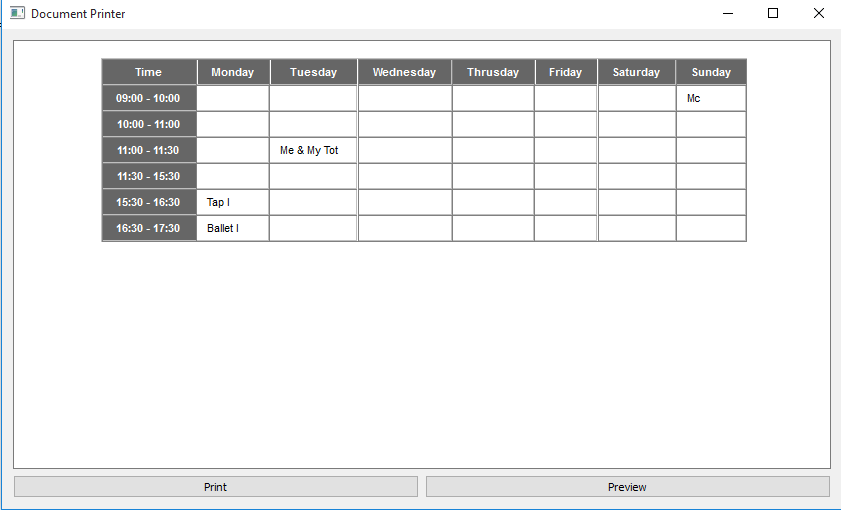
\includegraphics[width=\linewidth]{pics/userGuide/teacherSchedule.png}
  \caption{Teacher Schedule}
  \label{fig:User doc: Teacher Schedule}
\end{figure}


Class Role Sheet:\\
This button creates a window which contains the classes the logged in teacher is currently teaching. The user can click on a class to view the students in the class. If the user wants a formatted role sheet they can click the print button which allows the user to print out a role sheet for the class. The role sheet contains the students name, and emergency contact information, along with a check box for each week in a three month period. This format is accordance with the one a week classes offer at the Academy of Dance Arts.\\

\begin{figure}
  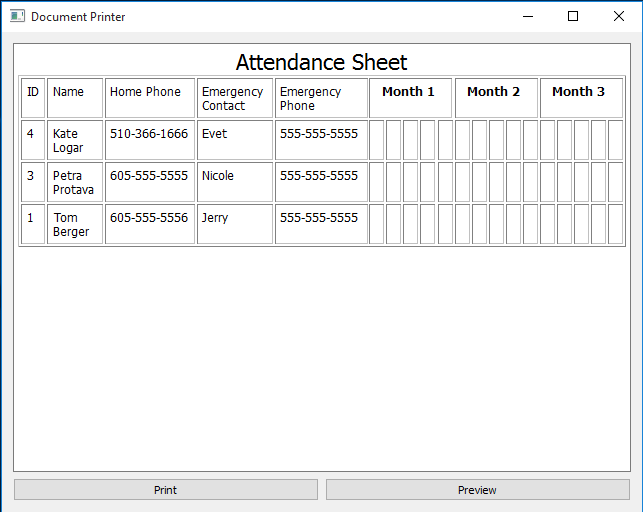
\includegraphics[width=\linewidth]{pics/userGuide/role.png}
  \caption{Class Role Sheet}
  \label{fig:User doc: Class Role Sheet}
\end{figure}

\subsubsection{Personal Options}
This section contains the functions connected to modify information directly connected to the user. These function include change password, change user name, modify personal information, and enter hours.

Change Password\\
When using this function the user is prompted with a dialog box, form this dialog the user will enter their user name, their desired new password, and confirm the new password. The user will be prompted to reenter their password if their user name or password are incorrect.\\

Change Username:\\
When using this function the user is prompted with a dialog box, form this dialog the user will enter their user name, their password, and the desired new user name. The user will be prompted to reenter their user name if their user name or password are incorrect.\\

Modify Personal Information:\\
If the user ever needs to change their personal information they can click this button to bring up a form containing their personal information. In this form the user can change their name, date of birth, phone numbers, address, and other information within the system. Like the other update teacher form in the admin section of the DanceSoft project, if the user leaves any of the required fields open they will be prompted to fill them in. Also if the user changes their address they will be given a dialog box asking if they would like to update their existing address or create a new one within the database. This is done because if two people going to, or working at the Academy live at the same address the teacher can create a new entry so that the other person address does not get effected. However if the teacher is the only one living at the address the system does not want to create dead data within the database, so the user is given an with an ability to change the entry. 

As stated the user should use caution when ever changing address because if a user updates an address that someone else lives at then that person will have incorrect data, also if a teacher is the only person in the database with an address and a new address is added instead of updating then dead data will be created, and in this project iteration a user would need to access the database directly to remove a dead address as address removal is linked to teacher and student removal.

Enter Hours:\\
The user is able to look through the pay rates linked to their account by system admin and log hours for the various pay rates.


\section{Installation Guide}
The following is the steps to install the DanceSoft software on a users machine:

\bf Step 1: \rm
	The first thing a user needs to do is make sure that a valid version of Python 3 can run on their system, if you already have python 3 installed on your machine please skip to step 2.
	The most recent version of Python 3 can be found on \url{https://www.python.org/downloads/} the user can then click on the download link and download a python zip file that is compatible with the operating system being used by the user.
	Follow the instruction on the install, one the install is complete the python files should be located in your local drive unless the user specified a different directory during install. A user has several ways of confirming that python installed correctly on their system. If the user is  with the command prompt they can run the Python 3 command to confirm successful installation. If the user would like to confirm using non-command line, the user can go to the python 3 file on their drive and run the Python.exe file. If a command window appears then the user has successfully installed python and can proceed to step 2.
	
\begin{figure}
  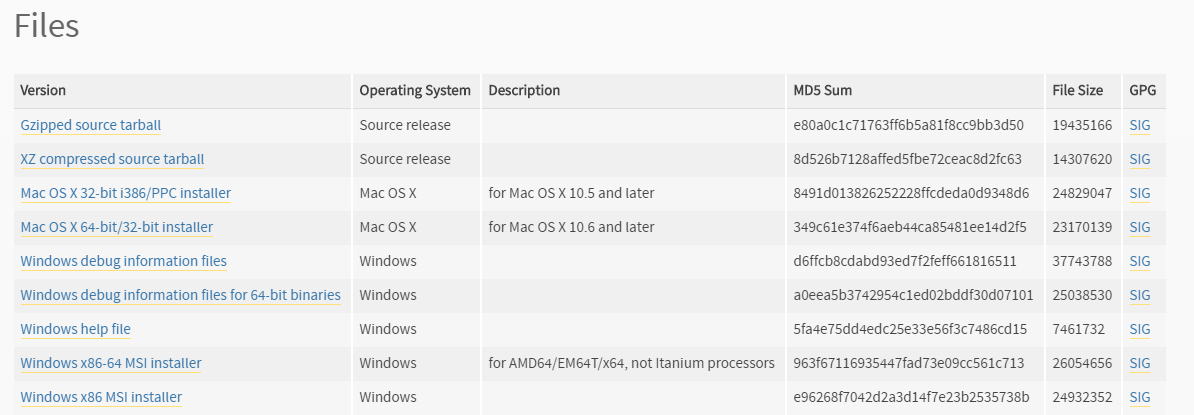
\includegraphics[width=\linewidth]{pics/pythonFiles.png}
  \caption{Python zip files}
  \label{fig:User doc: python files}
\end{figure}

\bf Step 2: \rm
	The next step is to install the PyQt libraries and the designer so the user can run the scripts containing PyQt code. There are several versions of PyQt, the version the DanceSoft team used was PyQt4. PyQt4 can be downloaded from \url{https://www.riverbankcomputing.com/software/pyqt/download}, one there the user can select the zip file that goes with their operating system. The website also provides stable windows installers if the user is running a windows system. If the installer is used the libraries will automatically be stored in the site-packages sub-directory of the python folder and the user should be able to start using PyQt libraries
	If the user is not running windows, they can download and use the brew facility to easily install the need files. If the user runs \bf brew install PyQt --with-python3 \rm from the OS X command line the system should automatically install the needed files.
	 Otherwise the user will need to download the snippets from \url{https://www.riverbankcomputing.com/software/pyqt/download} and install the PyQt libraries in the site-packages folder.
	 
\bf Step 3: \rm
	The last major install a user will need to do before using the software is the MySQL database software necessary to use the SQL components of the DanceSoft project.
	MySQL can be installed by following the download instructions on \url{https://www.mysql.com/downloads/} and downloading the free version of the software. This installer will install all the tools needed to manipulate and use the database directly if necessary.\\
	
The user should now have all the needed tools installed to run the DanceSoft Software.
	 
	


%% \newpage  %%  if needed ...
%\section{Programmer Manual}

